\documentclass{article}
\usepackage{graphicx}
\graphicspath{ {./images/} }
\usepackage{subfig}

\title{CTA200 Assignment 2 Question 3}
\author{Caleb Lammers}

\begin{document}
\maketitle

\section*{Question 1.}

\subsection*{Methods}

To create the graphs shown below, this program iterates
through points c, determining for each whether $\left| z \right|$ diverges
and plotting the point accordingly. In more detail, for $c = x + iy$, the
program starts with $x = -2 +$incr (for some small incr) and checks the
divergence of $\left| z \right|$ for $y = -2 +$incr, $y = -2 +2\cdot$incr,
$...$, $y = -2 +n\cdot$incr until $y = -2 +n\cdot$incr $>= 2$. Then, the
program repeats this whole process for $x = -2 + 2\cdot$incr and so on up until $x = -2 +
n\cdot$incr (note that it would be more efficient to use np.meshgrid, however, this is more intuitive). To check the divergence of $\left| z \right|$ for a given point c, the program
recursively calculates $z$ by $z_{i+1} = z_i^2 + c$ with $z_0$ = 0. If at some point in the
first 50 iterations $\left| z \right| > 10$ we conclude that $\left| z
\right|$ will diverge. In fact, this is actually overkill as it is well known
(and can be shown relatively easily) that if $\left| z \right| > 2$,
$\left| z \right|$ certainly diverges.\textsuperscript{1} The choice of 50
iterations is somewhat arbitrary but for high numbers of iterations there
are few difference in the image, due to the limited resolution (there are few
noticeable differences with 100 or even 1000 iterations). For higher resolution images, a smaller incr value is required, however, this increases the amount of computation.
Using matplotlib.pyplot, in graph 1, the points for which $\left| z \right|$ diverged were plotted in white and those which did not were coloured black. In the second graph, points for which $\left| z \right|$ did not diverge were again plotted in black but those that did were coloured using a colourmap according to the number of iterations until $\left| z \right| > 10$. The third graph was obtained by zooming into graph 2. \\

 1 - http://mathforum.org/library/drmath/view/68518.html

\newpage
\subsection*{Analysis}

\begin{figure}[h]
  \centering
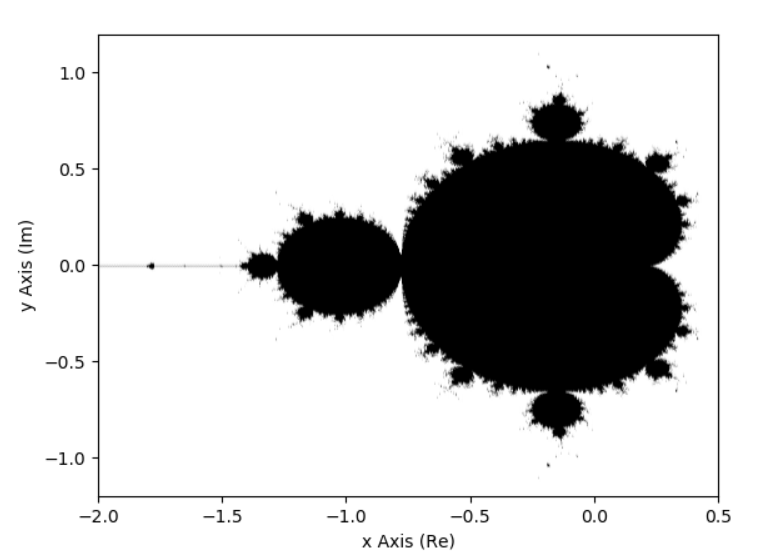
\includegraphics[scale=0.5]{Black and White}
\caption{Black and white graph (incr $ = 0.002$)}
\end{figure}

In the black and white graph, we can see that the points for which $\left| z
\right|$ did not diverge are around the origin, with most points having a negative
real part. With the recursive equation in mind, this makes sense as we are
repeatedly adding $c$. That is, if c itself has a very large magnitude, it is
clear that the recursion equation will diverge. As we are squaring $\left| z
\right|$, if $c$ has a negative real part, adding $c$ will decrease the magnitude of $z$
(as long as $z$ does not have too large of an imaginary part). Furthermore, even if you do not recognize this as the Mandelbrot set, it is visually clear that the graph has additional interesting properties. This is especially noticeable after colouring the diverging points.

\begin{figure}[h]
  \centering
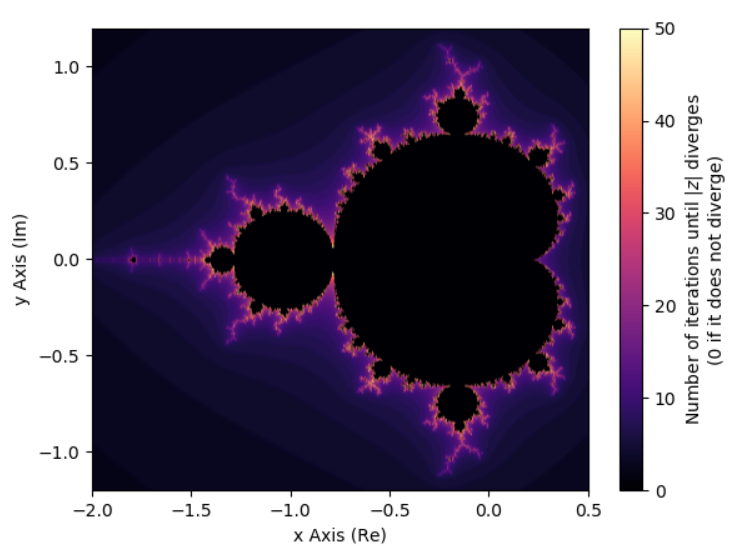
\includegraphics[scale=0.5]{Coloured}
\caption{Coloured graph (incr $ = 0.002$)}
\end{figure}

We see that a higher number of iterations is required to determine whether $\left| z \right|$ diverges for points near the perimeter of the figure and far fewer iterations are
required for points far from the perimeter, which is to be expected. Additionally, the coloured graph is quite aesthetically pleasing. One important observation to note is that it appears as though there are smaller copies of itself branching from the original shape.

\begin{figure}[h]
  \centering
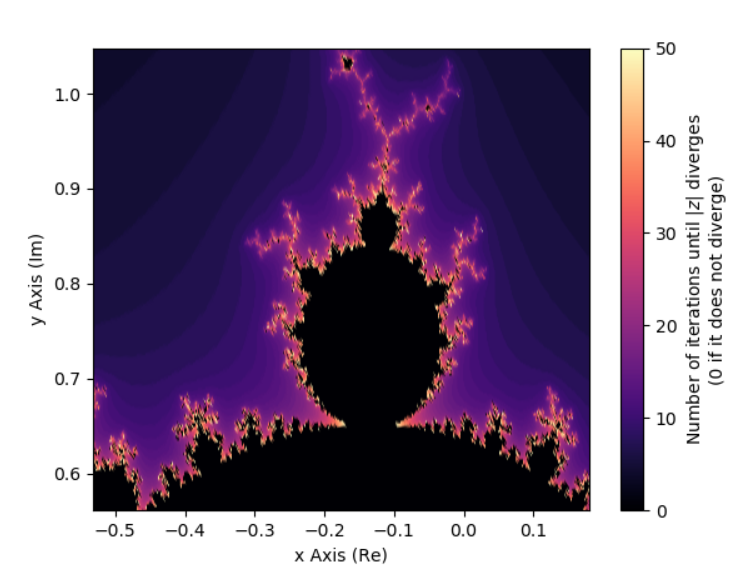
\includegraphics[scale=0.5]{Zoomed In}
\caption{Zoom in on Figure 2 (incr $ = 0.002$)}
\end{figure}

In the zoomed image, we can especially see the so-called "self-similarity" of
the Mandelbrot set that makes it a fractal. In fact, in this image we can even
see smaller similar shapes branching from itself again. This actually
continues indefinitely and there are many videos on the internet zooming into the
Mandelbrot set at a specific point to very high level of magnification. Indeed, the Mandelbrot set has became a staple of mathematical beauty.

\section*{Question 2.}

\subsection*{Methods}

Using the Scipy ODE solver and motivated choices of parameters, graphs
representing the idealized spreading of disease can be created. Using the SIR model
ODEs, the derivatives of $S$, $I$, and $R$ can each be calculated at time $t$.
By specifying $t_0$, $\beta$, $\gamma$, $t_{end}$, $dt$ and initial values for
$S$, $I$, and $R$, Scipy's ODE solver is used to numerically solve the
functions. Then, graphs are created using matplotlib.pyplot. From equation
(1), we see that $\beta$ is controlling the rate at which the number of
susceptible members of the population is decreasing. That is, roughly,
$\beta$ is controlling how infectious the disease is. In equation (2),
we see that $\gamma$ corresponds to the rate at which people people recover
from the disease. With these interpretations in mind, we will be able to choose
reasonable values for $\beta$ and $\gamma$ depending on the situation.
To incorporate deaths ($D$) into the model, notice that in this model recovered
and dead members of the population are analogous. So, the new equation is:
\[ \frac{dD}{dt} = \lambda I\]
Of course, the addition of this equation does not affect equation (3) or
equation (1) directly (which is clear by the analogy to equation (3)). However,
now we have \[ 1000 = S + I + R + D\]
\[\Rightarrow 0 = \frac{dS}{dt} +\frac{dI}{dt} + \frac{dR}{dt} + \frac{dD}{dt}\]
\[\Rightarrow \frac{dI}{dt} = \frac{\beta S I}{N}  - \gamma I - \lambda I\]

This makes sense, as people who die from the disease can no longer spread the
disease, which should decrease $I$.

\subsection*{Analysis}

Depending on the values of $\beta$ and $\gamma$, over the course of $t = 0$ to
$t = 200$, varying proportions of the population will be infected and
recover/not recover.

\begin{figure}[htbp]
\centering
\subfloat[$\beta = 0.3, \gamma = 0.2$]{\label{fig:a}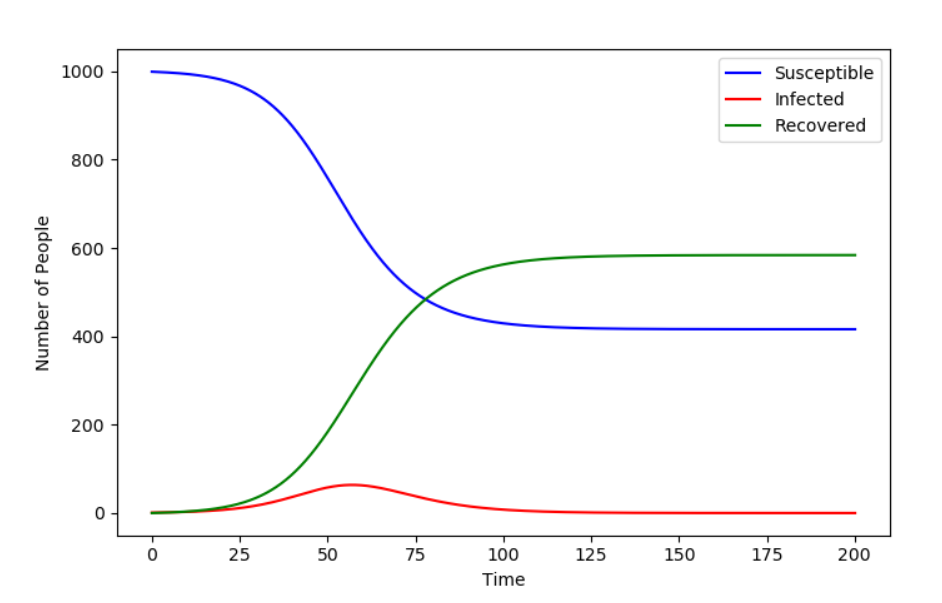
\includegraphics[width=0.46\linewidth]{Graph 1}}\qquad
\subfloat[$\beta = 0.4, \gamma = 0.03$]{\label{fig:b}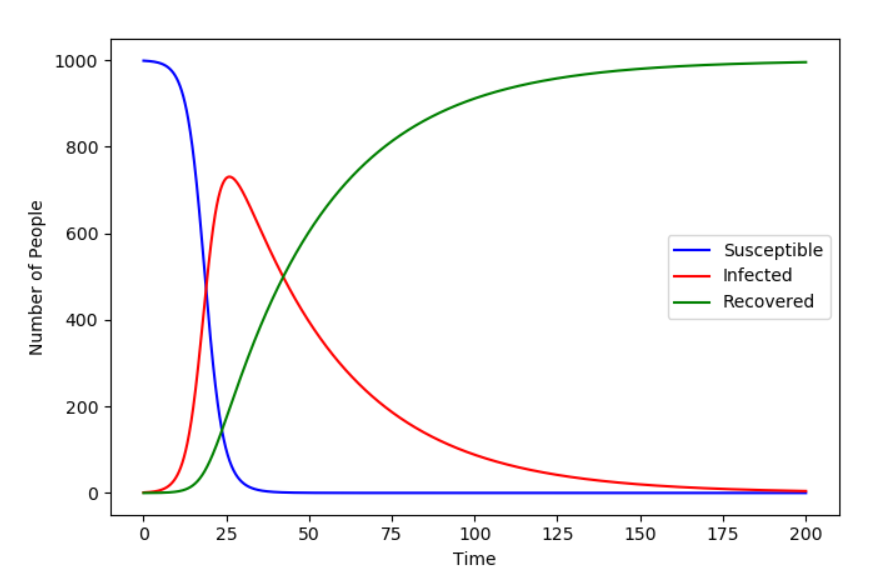
\includegraphics[width=0.46\linewidth]{Graph 2}}\\
\subfloat[$\beta = 0.3, \gamma = 0.01$]{\label{fig:c}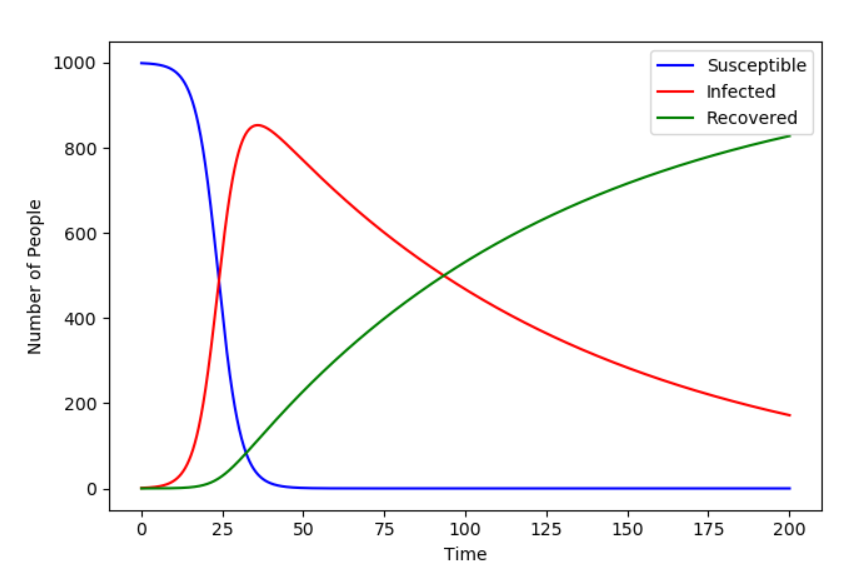
\includegraphics[width=0.46\textwidth]{Graph 3}}\qquad
\subfloat[$\beta = 0.05, \gamma = 0.01$]{\label{fig:d}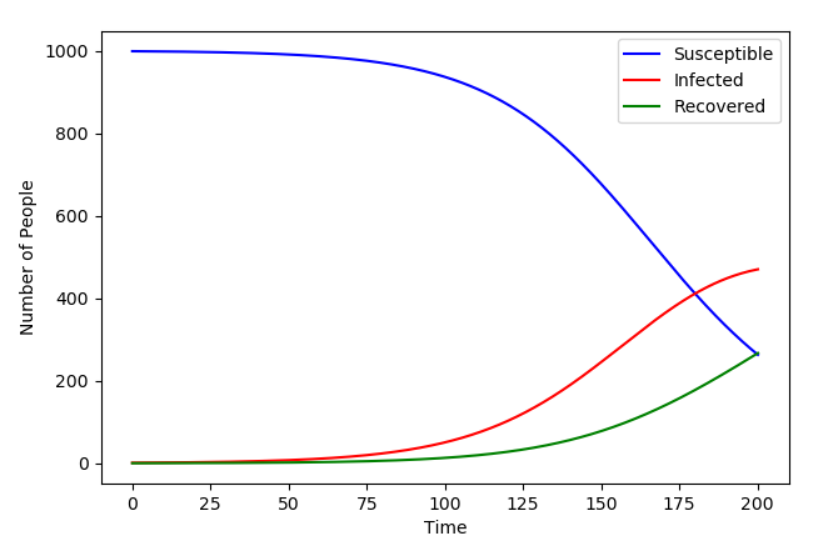
\includegraphics[width=0.46\textwidth]{Graph 4}}
\caption{Plots of S, I, and R for different motivated $\beta$ and $\gamma$}
\label{fig:myfig}
\end{figure}

Different physical situations require varying values of $\beta$ and $\gamma$.
Figure 4. a) depicts a disease that has a high recovery rate and a somewhat low
infection rate. This is modelled by a medium $\beta$ and a relatively high
$\gamma$. Figure 4. b) shows a disease that has a high infection rate and a
recovery rate that is high enough for everyone to recover but low enough that
everyone is infected. This type of disease requires a relatively high $\beta$ and a medium $\gamma$. Next, Figure 4. c) represents a disease with a somewhat high infection rate but
a low recovery rate, modelled with a medium $\beta$ and a small $\gamma$.
Lastly, Figure 4. d) shows a disease with a low infection rate and a low
recovery rate, which requires a low $\beta$ and $\gamma$. Of course, there are
many other examples of physically possible situations that each require their own modifications to $\beta$ and $\gamma$.

\begin{figure}[h]
  \centering
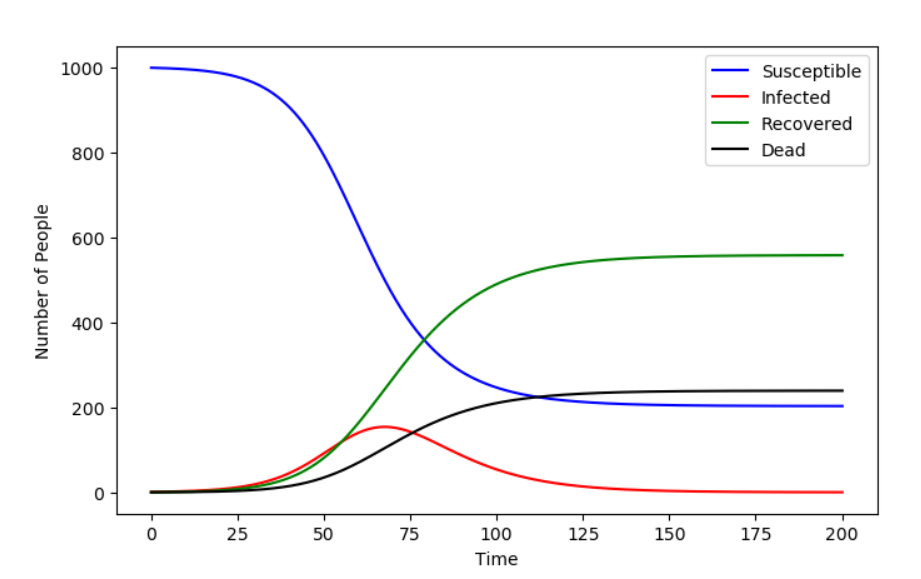
\includegraphics[scale=0.4]{Graph 5}
\caption{Plot including deaths with $\beta = 0.2, \gamma = 0.07 \lambda = 0.03$}
\end{figure}

When also considering deaths, there even more possible circumstances. Above is the
graph of a disease with a relatively low infection rate, high recovery rate,
and medium mortality rate (the parameters required are as you would expect). Despite starting with idealized equations, it is interesting to see the utility they provide in modelling something as complex as the spread of a disease.


\end{document}
